% Logic Analyzer with Live Protocol Decoding
% Class report formatted with the HardwareX article template (Version 2, June 2021).
% Build variants:
%   hardwarex-embedded.tex  Lingga Aradhana Sahadewa only
%   hardwarex-fpga.tex      Lingga Aradhana Sahadewa, Alvin Hadar, Bagas Budhi Permana
\documentclass[11pt,a4paper]{article}
\usepackage[utf8]{inputenc}
\usepackage[margin=1.5cm]{geometry}
\usepackage{titlesec}
\usepackage{array}
\usepackage{tabularx}
\usepackage{longtable}
\usepackage{enumitem}
\usepackage{amssymb}
\usepackage{xcolor}
\usepackage{lmodern}
\usepackage{graphicx}
\usepackage{float}
\usepackage{textcomp}
\usepackage{hyperref}
\usepackage{xurl}
% Break paths and URLs at natural separators only.
\def\UrlBreaks{\do\/\do\.\do\-\do\_}
\hypersetup{
    colorlinks=true,
    linkcolor=blue,
    filecolor=magenta,
    urlcolor=blue,
}
\urlstyle{same}

\titleformat{\section}[block]{\hspace{1em}\bfseries}{\thesection.}{0.5em}{}
\titleformat{\subsection}[block]{\hspace{1em}}{\thesubsection}{0.5em}{}

\setlength{\parindent}{0pt}
\setlength{\parskip}{8pt}
\setlength{\emergencystretch}{3em}
\setlength{\tabcolsep}{4pt}
\renewcommand{\arraystretch}{1.15}
\setlength{\LTleft}{0pt}
\setlength{\LTright}{0pt}

% \code detokenizes identifiers so underscores and paths need no manual escaping.
\newcommand{\code}[1]{\texttt{\detokenize{#1}}}
\newcommand{\iu}{I\textsuperscript{2}C}

\providecommand{\ReportAuthorNames}{Lingga Aradhana Sahadewa, Alvin Hadar, Bagas Budhi Permana}
\newif\ifFPGA
\ifdefined\ReportFpgaVariant
  \FPGAtrue
\else
  \FPGAfalse
\fi

\begin{document}

\begin{flushleft}
{\LARGE\bfseries Logic Analyzer with Live Protocol Decoding}\\[0.35cm]
\textbf{Authors}\\
\ReportAuthorNames\\[0.25cm]
\textbf{Corresponding author email address}\\
\href{mailto:linggaaradhanas@gmail.com}{linggaaradhanas@gmail.com}\\[0.25cm]
\textbf{Class project}\\
\ifFPGA
FPGA class, 15 September--12 October 2026.
\else
Embedded system class, 15 September--12 October 2026.
\fi
Funded by the Korea Chamber of Commerce and Industry (KCCI).
\end{flushleft}

\vspace{0.2cm}
\textbf{Abstract}\\
This project develops an eight-channel logic analyzer on the Zybo Z7-10 for
observing 3.3~V digital signals. The FPGA samples at up to 100 million samples
per second (MS/s), detects trigger conditions, and records data before and after
a trigger. Direct memory access (DMA) transfers the samples to DDR memory.
FreeRTOS runs on the Zynq Cortex-A9 processor and coordinates acquisition,
protocol decoding, commands, and USB communication. Separate tasks exchange
buffer references through queues so that decoding cannot read a buffer while
DMA overwrites it. Three decoder tasks support configurable UART, SPI, and
\iu{} analysis. A Windows-hosted browser interface displays captured waveforms
and live decoded events. In three USB transfer trials, each trial transferred
sixteen 4~MiB captures at 1.62~MB/s with exact data agreement. A separate
60-second UART test delivered 606,411 events without dropped segments or
client-side event loss. The results demonstrate high-speed buffered acquisition
and lower-rate live analysis. The main capacity limits are decoder throughput,
available memory, and USB transfer speed.

\vspace{0.2cm}
\textbf{Keywords}\\
Logic analyzer; FPGA; FreeRTOS; protocol decoding; USB; embedded systems

\newpage
\textbf{Specifications table}\\
\vskip 0.2cm
\begin{tabularx}{\linewidth}{|>{\raggedright\arraybackslash}p{4.5cm}|>{\raggedright\arraybackslash}X|}
\hline
\textbf{Hardware name} & Logic Analyzer with Live Protocol Decoding \\ \hline
\textbf{Video demonstration} &
\href{https://youtu.be/1xx84Ndi4vQ?si=ldsuYEWvYVqu2u6-}{\texttt{youtu.be/1xx84Ndi4vQ}} \\ \hline
\textbf{Subject area} & Digital electronics, FPGA design, and real-time embedded systems \\ \hline
\textbf{Hardware type} & Digital logic analyzer with protocol decoding \\ \hline
\textbf{Comparable instruments} & Saleae Logic family and Digilent Digital
Discovery \\ \hline
\textbf{Cost of hardware} & Rp 13,954,700 for the required USB build, estimated
on 17 September 2026 \\ \hline
\textbf{Input channels} & Eight 3.3~V LVCMOS33 channels on Pmod JC (CH0--CH7),
plus common ground \\ \hline
\textbf{Sample rate} & Up to 100~MS/s; rate = 100~MHz / (\code{SAMPLE_DIV} + 1) \\ \hline
\textbf{Trigger} & Level and edge conditions, pre/post-trigger capture, timeout
and abort \\ \hline
\textbf{Pre-trigger configuration} & Up to 32,768 samples; the internal ring has
65,536 entries \\ \hline
\textbf{Encoding} & Four eight-bit raw samples per 32-bit word, or 24-bit run
plus eight-bit sample \\ \hline
\textbf{Capture storage} & 8~MiB burst pool; live mode reuses the first 4~MiB as
16 $\times$ 256~KiB segments \\ \hline
\textbf{DMA} & AXI DMA S2MM, ordinary scatter-gather descriptors; hardware cyclic
mode disabled \\ \hline
\textbf{RTOS} & FreeRTOS on CPU0, 1~kHz tick, statically allocated application
objects \\ \hline
\textbf{Default connection} & Direct Zynq PS USB0 CDC-ACM through J10; Windows
\texttt{usbser.sys} \\ \hline
\textbf{Protocol decoders} & UART, SPI and \iu{}; three independently
configurable live slots \\ \hline
\textbf{Host applications} & \code{la-ui} browser workspace and \code{la-cli}
scripted interface \\ \hline
\textbf{Exports} & PulseView \code{.sr}, VCD, sample/event CSV, PNG and text
through the applicable host tools \\ \hline
\textbf{Data integrity} & CRC16 per protocol frame; CRC32 and size/order checks
per completed capture \\ \hline
\end{tabularx}

\section{Hardware in context}

Embedded communication faults are difficult to diagnose from software messages
alone. A UART byte can be wrong because of timing or baud configuration; an SPI
transfer can fail because of clock polarity or chip-select timing; an \iu{}
transaction can fail because an address was not acknowledged. A logic analyzer
records the digital waveforms and associates protocol events with their sample
positions, allowing the signal behavior to be compared with the intended
transaction.

The project combines FPGA design and real-time embedded software in one
measurement instrument. The FPGA handles precise sampling and triggering.
The processor configures captures, decodes communication protocols, and sends
results to the computer. This division lets the instrument sample signals much
faster than software could process individual inputs. Commercial instruments
such as the Saleae Logic family and Digilent Digital Discovery provide similar
measurement functions. The project also exports files for sigrok/PulseView.

The initial design sent data through an ESP32 Wi-Fi gateway. Transport
limitations led to a direct USB connection between the Zynq and the computer.
USB became the default connection in September. The browser interface runs on
the computer and communicates with the analyzer through a local host application.
The older gateway remains available as an optional configuration.

\subsection{Project scope and division of work}

\begin{longtable}{|>{\raggedright\arraybackslash}p{2.4cm}|>{\raggedright\arraybackslash}p{7.0cm}|>{\raggedright\arraybackslash}p{7.4cm}|}
\hline
\textbf{Area} & \textbf{Design work} & \textbf{Implementation and verification} \\ \hline
\endhead
FPGA & Synchronizing inputs, setting the sample rate, detecting triggers,
retaining pre-trigger samples, packing data, and generating test signals.
Verification includes RTL simulation and routed timing/resource analysis. &
\path{fpga/rtl/}, \path{fpga/tb/}, \path{fpga/scripts/},
\path{docs/regmap.yaml}, Vivado reports \\ \hline
Embedded system & Scheduling FreeRTOS tasks, exchanging commands and buffer
references, decoding UART/SPI/\iu{}, and transferring results over USB.
Verification includes data-integrity and overload-recovery tests. &
\path{fw-zynq/app/src/}, \path{common/la_decode/}, \path{common/la_proto/},
\path{host/}, RTOS and bench reports \\ \hline
Shared integration & Connecting FPGA registers and DMA to the firmware,
checking captured data, displaying live results, and starting the instrument
from an SD card. &
\path{docs/architecture.md}, \path{docs/rtos-design.md}, \path{docs/status.md}
and the operator runbook \\ \hline
\end{longtable}

The FPGA and embedded software form a single acquisition pipeline. Registers
carry configuration commands to the FPGA, while DMA transfers captured samples
to memory for software processing. This interface connects the sampling hardware
to the RTOS tasks described in Section~\ref{sec:rtos}.

\ifFPGA
Alvin Hadar developed the RTL capture FIFO/buffer and sample packing. Bagas
Budhi Permana developed trigger and edge detection with AXI-Stream packet
framing. Lingga Aradhana Sahadewa was responsible for the remaining design work,
embedded software, host software, integration, testing, and documentation.
\fi

\section{Hardware description}

Figure~\ref{fig:system} shows the signal path from the target circuit to the
computer. The FPGA captures the inputs, DMA writes the data to memory, and
FreeRTOS tasks process the data before USB transmission.

Figure~\ref{fig:hardware-photo} shows the assembled instrument on the bench.
The Zybo Z7-10 provides the FPGA, ARM processor, DDR memory, and USB interfaces.
Jumper leads connect the acquisition header to the circuit under test.

\begin{figure}[htbp]
\centering
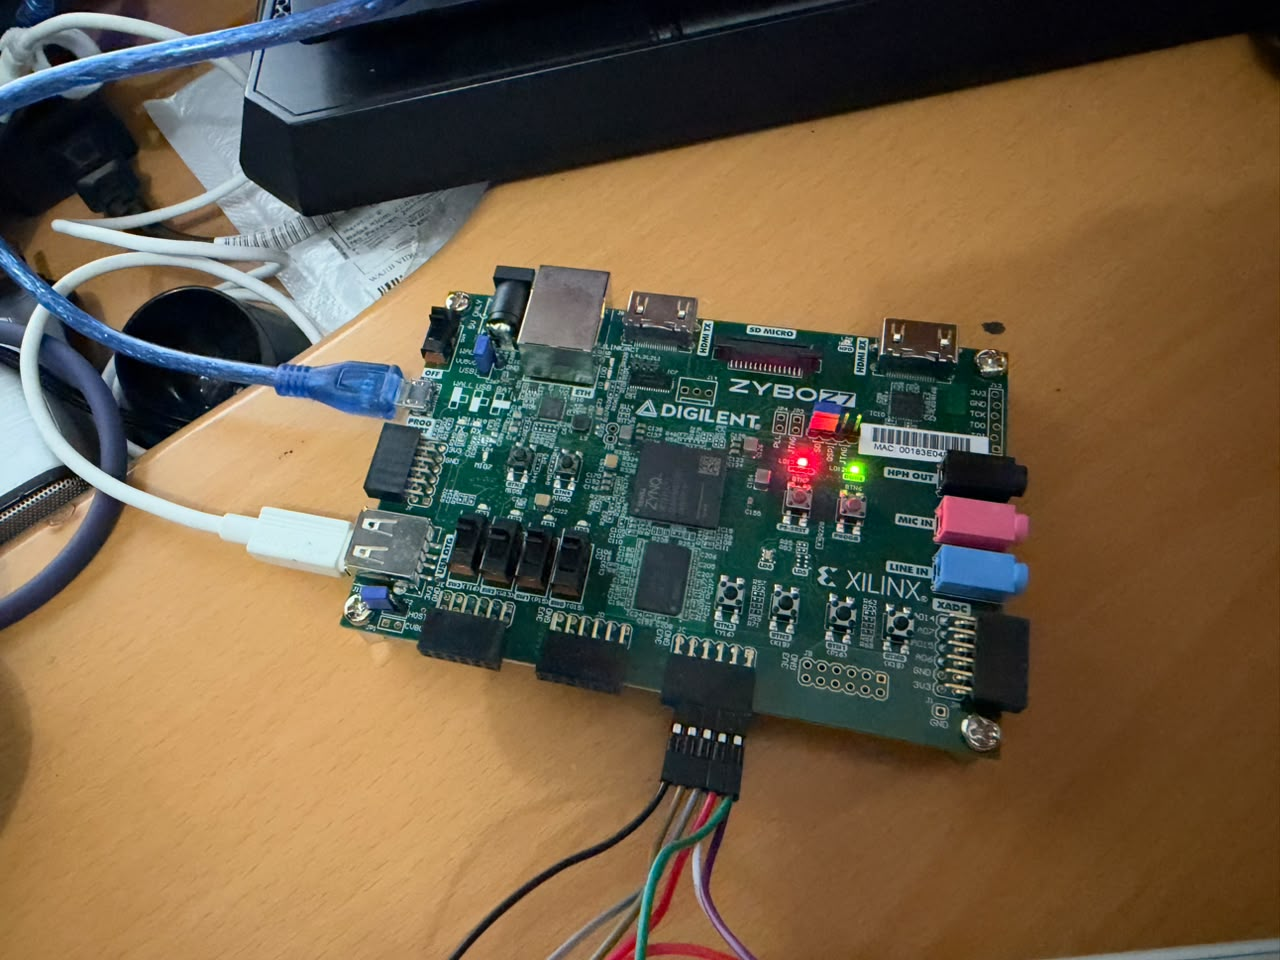
\includegraphics[width=0.70\linewidth]{../assets/logic-analyzer-hardware.jpeg}
\caption{Logic analyzer hardware assembly on the Zybo Z7-10. The photograph
shows the powered development board, USB connections, and acquisition leads.}
\label{fig:hardware-photo}
\end{figure}

\begin{figure}[htbp]
\centering
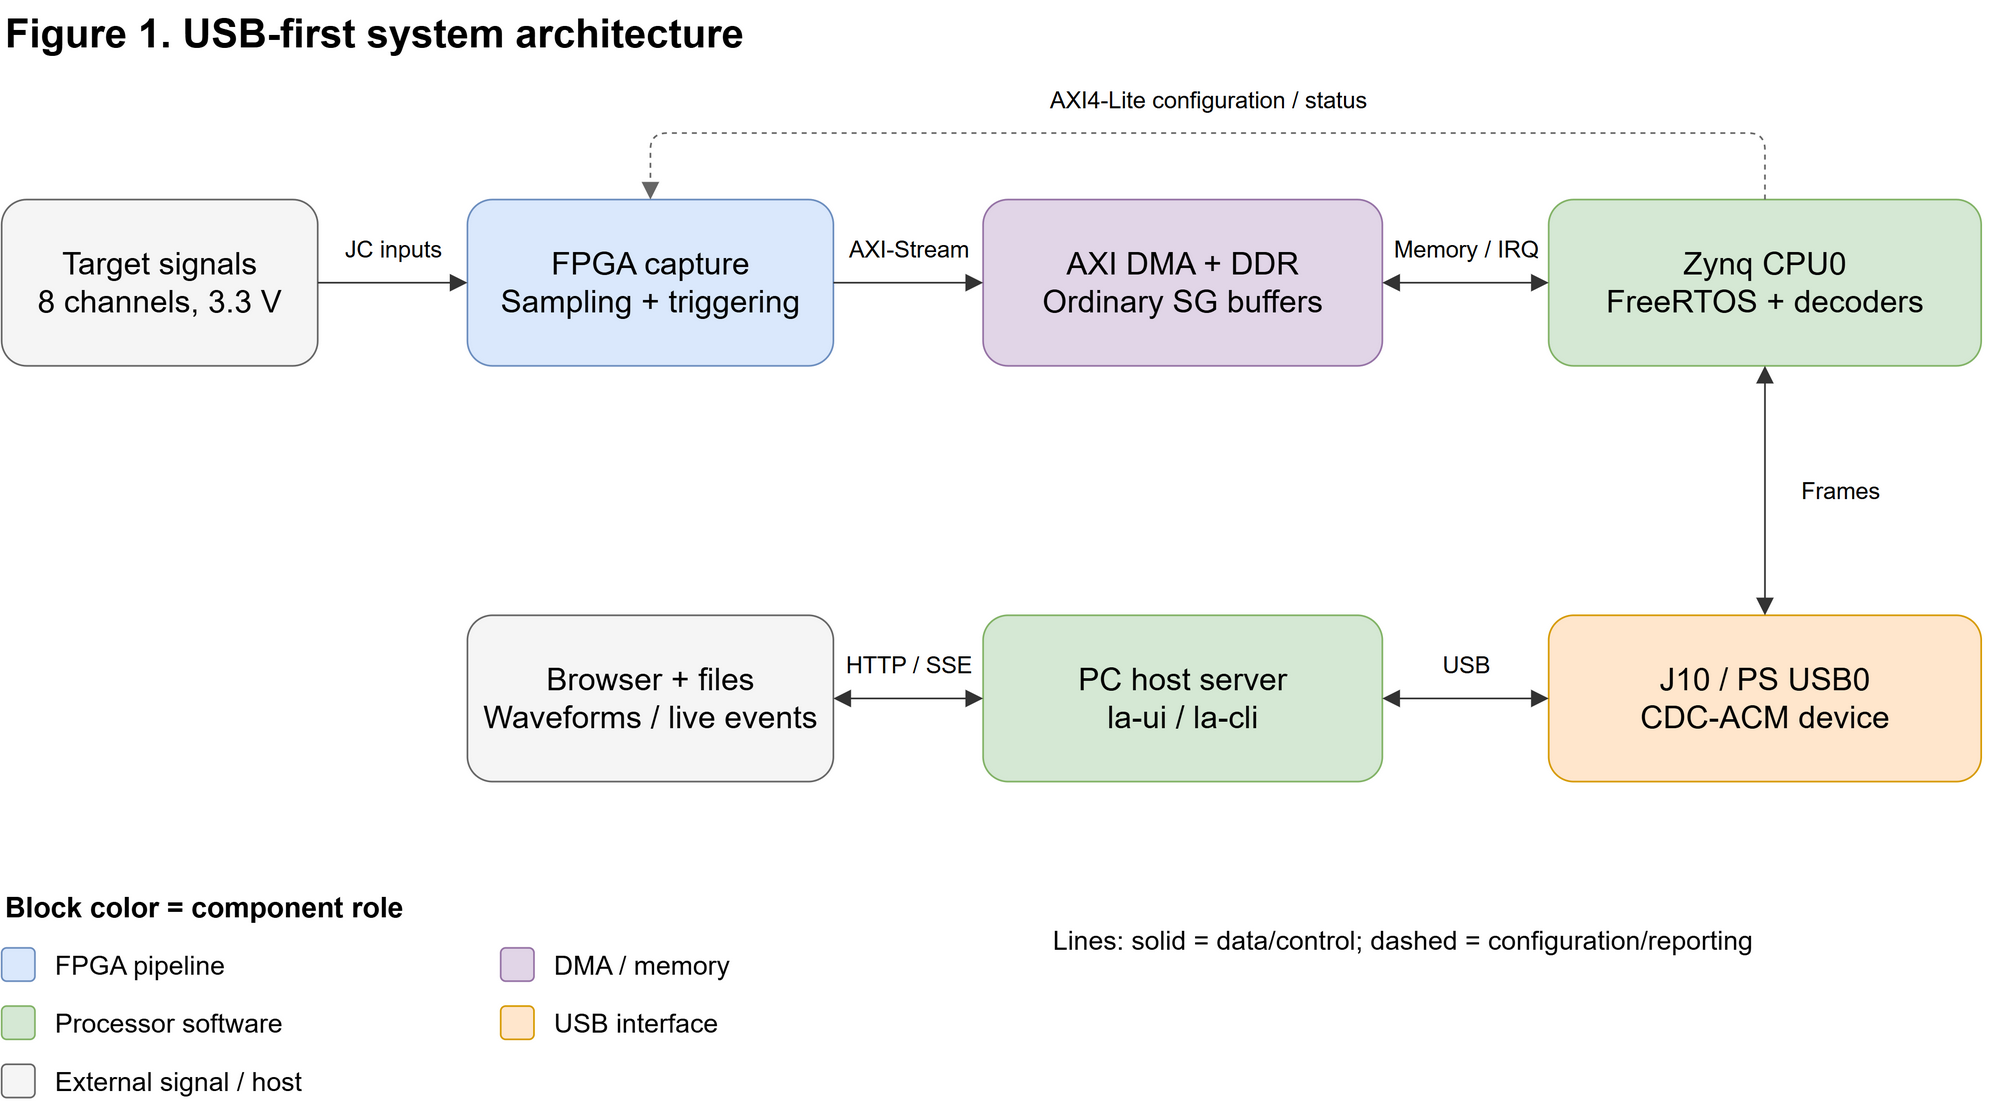
\includegraphics[width=\linewidth]{../assets/figures/01-system.png}
\caption{System architecture. Signals enter through JC and pass through the
FPGA capture logic, DMA, DDR memory, and processor before reaching the PC through
J10 USB. AXI4-Lite registers carry control and status information. The local
host server connects the browser to the device.}
\label{fig:system}
\end{figure}

\subsection{FPGA subsystem}

The FPGA design is written as register-transfer-level (RTL) modules in
SystemVerilog. AXI4-Lite provides processor-readable control and status registers.
AXI-Stream carries captured data toward DMA. Unlike the register interface,
the stream interface transfers a sequence of data words with ready/valid
handshaking between sender and receiver.

\begin{figure}[htbp]
\centering
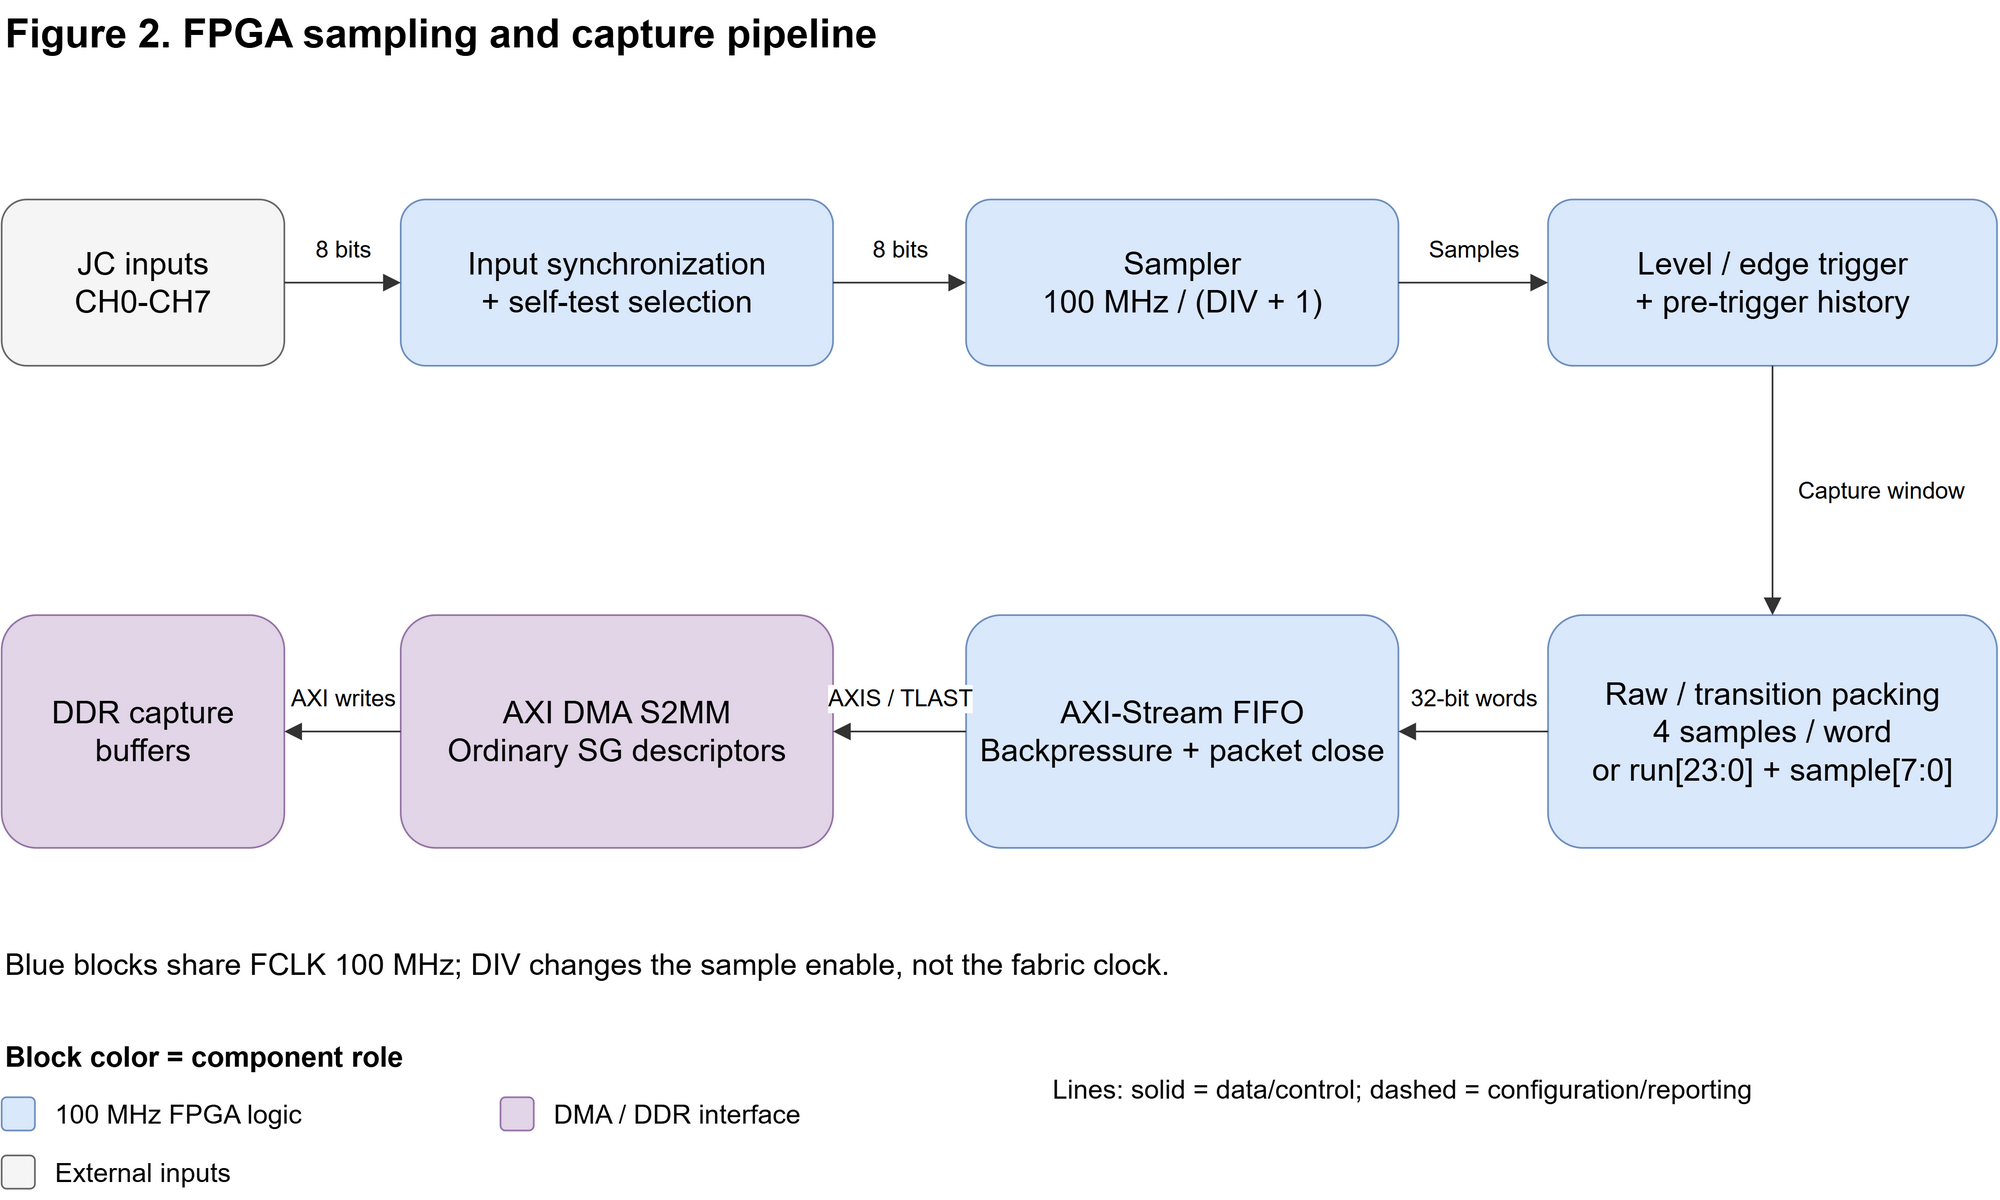
\includegraphics[width=\linewidth]{../assets/figures/02-fpga.png}
\caption{The custom capture logic shares the 100~MHz fabric clock. Sample-rate
division changes the sampling enable. Packing produces 32-bit words, and the
AXI-stream packet boundary tells the DMA when the captured packet is complete.}
\label{fig:fpga}
\end{figure}

The input signals are asynchronous to the FPGA clock. \code{la_input_sync}
synchronizes them before \code{la_sampler} records a sample at the configured
interval. Each sample contains the states of all eight channels in one byte.
For self-tests, a multiplexer selects the internal pattern generator instead of
the external inputs.

\code{la_trigger} checks selected channels for a level or edge condition.
\code{la_pretrig_ring} continuously retains recent samples so that the capture
can include activity before the trigger. Once the trigger occurs, the capture
controller records the requested remaining samples and closes the capture.
It also handles abort requests and FIFO overflow.

Two encodings are available. Raw encoding stores four sample bytes in each
32-bit word. Transition encoding stores an eight-bit signal value and a 24-bit
count of consecutive samples with that value. This reduces storage for signals
that remain unchanged for many samples. An AXI-Stream FIFO temporarily holds
output when DMA cannot accept it. The final transfer carries the TLAST signal
to mark the packet boundary.

The pattern generator provides counter, walking-one, PRBS8, UART, SPI and \iu{}
stimulus. Internal self-test exercises the acquisition pipeline; JE-to-JC
external loopback additionally exercises the physical pads and input
synchronizers. These are distinct validation paths.

The AXI-Lite register source is \path{docs/regmap.yaml}. Its C, SystemVerilog and
Markdown views are generated rather than hand-maintained. The control block is
mapped at 0x40000000 and DMA control at 0x40400000 in the integrated design.

\subsection{DMA, DDR and operating modes}

DMA transfers FPGA output to DDR memory without making the processor copy each
sample. A scatter-gather (SG) descriptor tells DMA where a destination buffer
starts and how much data it can hold. Multiple descriptors link these buffers
into a transfer sequence.

In burst mode, AcqTask prepares a finite descriptor chain for one capture.
After acquisition completes, TxTask sends the stored samples to the computer.
In live mode, DMA writes transition packets into sixteen 256~KiB memory segments.
Decoder tasks process completed segments while acquisition continues in other
segments. A packet closes after two milliseconds or at its configured size limit,
whichever occurs first. Software uses the actual written length, which can be
smaller than the segment capacity.

Both modes use ordinary scatter-gather descriptors with hardware cyclic mode
disabled. In live mode, software returns a segment to DMA only after its
consumers finish reading it. Descriptors occupy non-cacheable memory. Sample
buffers use cache maintenance so that the processor reads the data DMA most
recently wrote.

At 100~MS/s, raw acquisition is 100~MB/s because each sample is one byte. That is
not the sustained PC transfer rate. The current USB drain measurement is
1.62~MB/s, so full-rate acquisition uses finite buffers. Transition encoding
reduces low-transition captures, but its worst case can expand to four bytes per
sample. Loss-free continuous operation is bounded by both decoding and transport
capacity.

\subsection{USB and host subsystem}

The Zynq processing-system (PS) USB0 controller uses the onboard USB physical
interface and J10 device connector. Its CDC-ACM serial-device interface allows
Windows to expose the analyzer as a COM port through
\texttt{usbser.sys}. The USB-profile image does not initialize the gateway UART0
link or the PL SPI-bulk service. J12 supplies the documented board
power/JTAG/console path; J10 carries analyzer data.

\code{la-ui} supplies connection controls, captures, waveform viewing, cursors
and edge stepping, host-side recorded-capture decoding, per-slot live control,
exports, offline opening, traces and pattern-generator controls. \code{la-cli}
provides the corresponding scripted operations. Live events come from the
device decoder tasks; decoding an existing capture uses the host native decoder
library. The host forwards live events to the browser through server-sent events
(SSE), a persistent HTTP connection. One host connection owner
prevents competing operations from claiming the same COM port.

\subsection{Real-time operating system design}
\label{sec:rtos}

\subsubsection{Why FreeRTOS is used}

The real-time operating system (RTOS) controls when each software task runs.
Several software activities must progress during a measurement. New samples
arrive from DMA, decoders process earlier samples, and USB sends previous results
to the computer. Meanwhile, the instrument must still accept Stop, Abort, and
configuration commands. FreeRTOS divides these activities into separate tasks
on Zynq CPU0. A task waits when it has no work, allowing another ready task to
use the processor.

The scheduler uses a one-millisecond tick to manage task timing and timeouts.
This tick does not determine the sampling interval. At 100~MS/s, the FPGA takes
one sample every ten nanoseconds. DMA collects those samples in memory, and
FreeRTOS tasks process completed groups of data. Hardware therefore maintains
sample timing even when the processor switches between software tasks.

At startup, \code{main.c} checks reserved memory and the FPGA register interface,
then sets memory and cache attributes. \code{la_app_init()} creates the tasks,
queues, and buffers before \code{vTaskStartScheduler()} starts scheduling.
These application objects use statically allocated memory, so their storage is
reserved before acquisition begins.

The scheduler is preemptive: a ready task with a higher priority can interrupt a
lower-priority task. Ready tasks at the same priority share processor time through
time slicing. A task blocked on a queue or notification consumes no processing
time until data arrives or its timeout expires.

\subsubsection{Task responsibilities and priorities}

\begin{longtable}{|>{\raggedright\arraybackslash}p{3.0cm}|>{\raggedright\arraybackslash}p{1.3cm}|>{\raggedright\arraybackslash}p{1.3cm}|>{\raggedright\arraybackslash}p{10.8cm}|}
\hline
\textbf{Task} & \textbf{Prio.} & \textbf{Stack} & \textbf{Function} \\ \hline
\endhead
AcqTask / \code{la_acq} & 6 & 4~KiB & Starts and stops acquisition, checks
completed DMA transfers, and returns released buffers to DMA. Waits for control,
hardware-completion, or buffer-release notifications. \\ \hline
CmdTask / \code{la_cmd} & 5 & 4~KiB & Reads received bytes, checks command
frames, and forwards requests and acknowledgements to the appropriate task. \\ \hline
TxTask / \code{la_tx} & 5 & 12~KiB & Packages captures and decoded events for
transmission. Handles acknowledgements and retransmissions, then releases used
event blocks. \\ \hline
Decoder slot 0 / \code{la_dec0} & 5 & 4~KiB & Waits for sample segments,
decodes the selected protocol, and queues blocks of decoded events. \\ \hline
Decoder slot 1 / \code{la_dec1} & 5 & 4~KiB & Same independently configurable
role for slot 1 \\ \hline
Decoder slot 2 / \code{la_dec2} & 5 & 4~KiB & Same independently configurable
role for slot 2 \\ \hline
UsbTask / \code{la_usb} & 5 & 12~KiB & Services the USB connection, forwards
received bytes, and sends queued frames in order. Wakes on a notification or
after a 1~ms timeout. \\ \hline
StatusTask / \code{la_status} & 1 & 4~KiB & Checks remaining stack space for
the monitored tasks every five seconds. \\ \hline
\end{longtable}

There are eight application tasks in the default USB build, plus FreeRTOS idle
and timer tasks. The three decoder slots are not hard-wired one each to UART, SPI
and \iu{}: any supported configuration can be assigned to a slot, or that slot
can be disabled. Stack constants in \code{la_app.h} count 32-bit stack elements:
1024 elements are 4~KiB, and 3072 elements are 12~KiB. Idle and timer stacks are
separately 2~KiB each.

Higher priority numbers indicate greater urgency. Each stack holds a task's
local variables and saved function state while another task runs. The idle task
runs when no application task is ready, and the timer task services FreeRTOS
software timers.

AcqTask has the highest application priority because completed DMA buffers need
prompt attention. It checks completed transfers and makes their data available
to consumers, then waits for the next notification. Decoding and USB transmission
run at priority 5 because they can take longer and must share CPU time with
command processing.

An earlier priority assignment placed TxTask below the decoders. Under sustained
input, the ready decoder tasks prevented TxTask from sending their results.
Raising TxTask to priority 5 let production and transmission progress together.
Each decoder processes at most four segments per turn, and the transmitter
handles at most four live event blocks per turn. These limits help it return
regularly to command and stop handling.

\subsubsection{From a UART signal to a displayed event}

\begin{figure}[H]
\centering
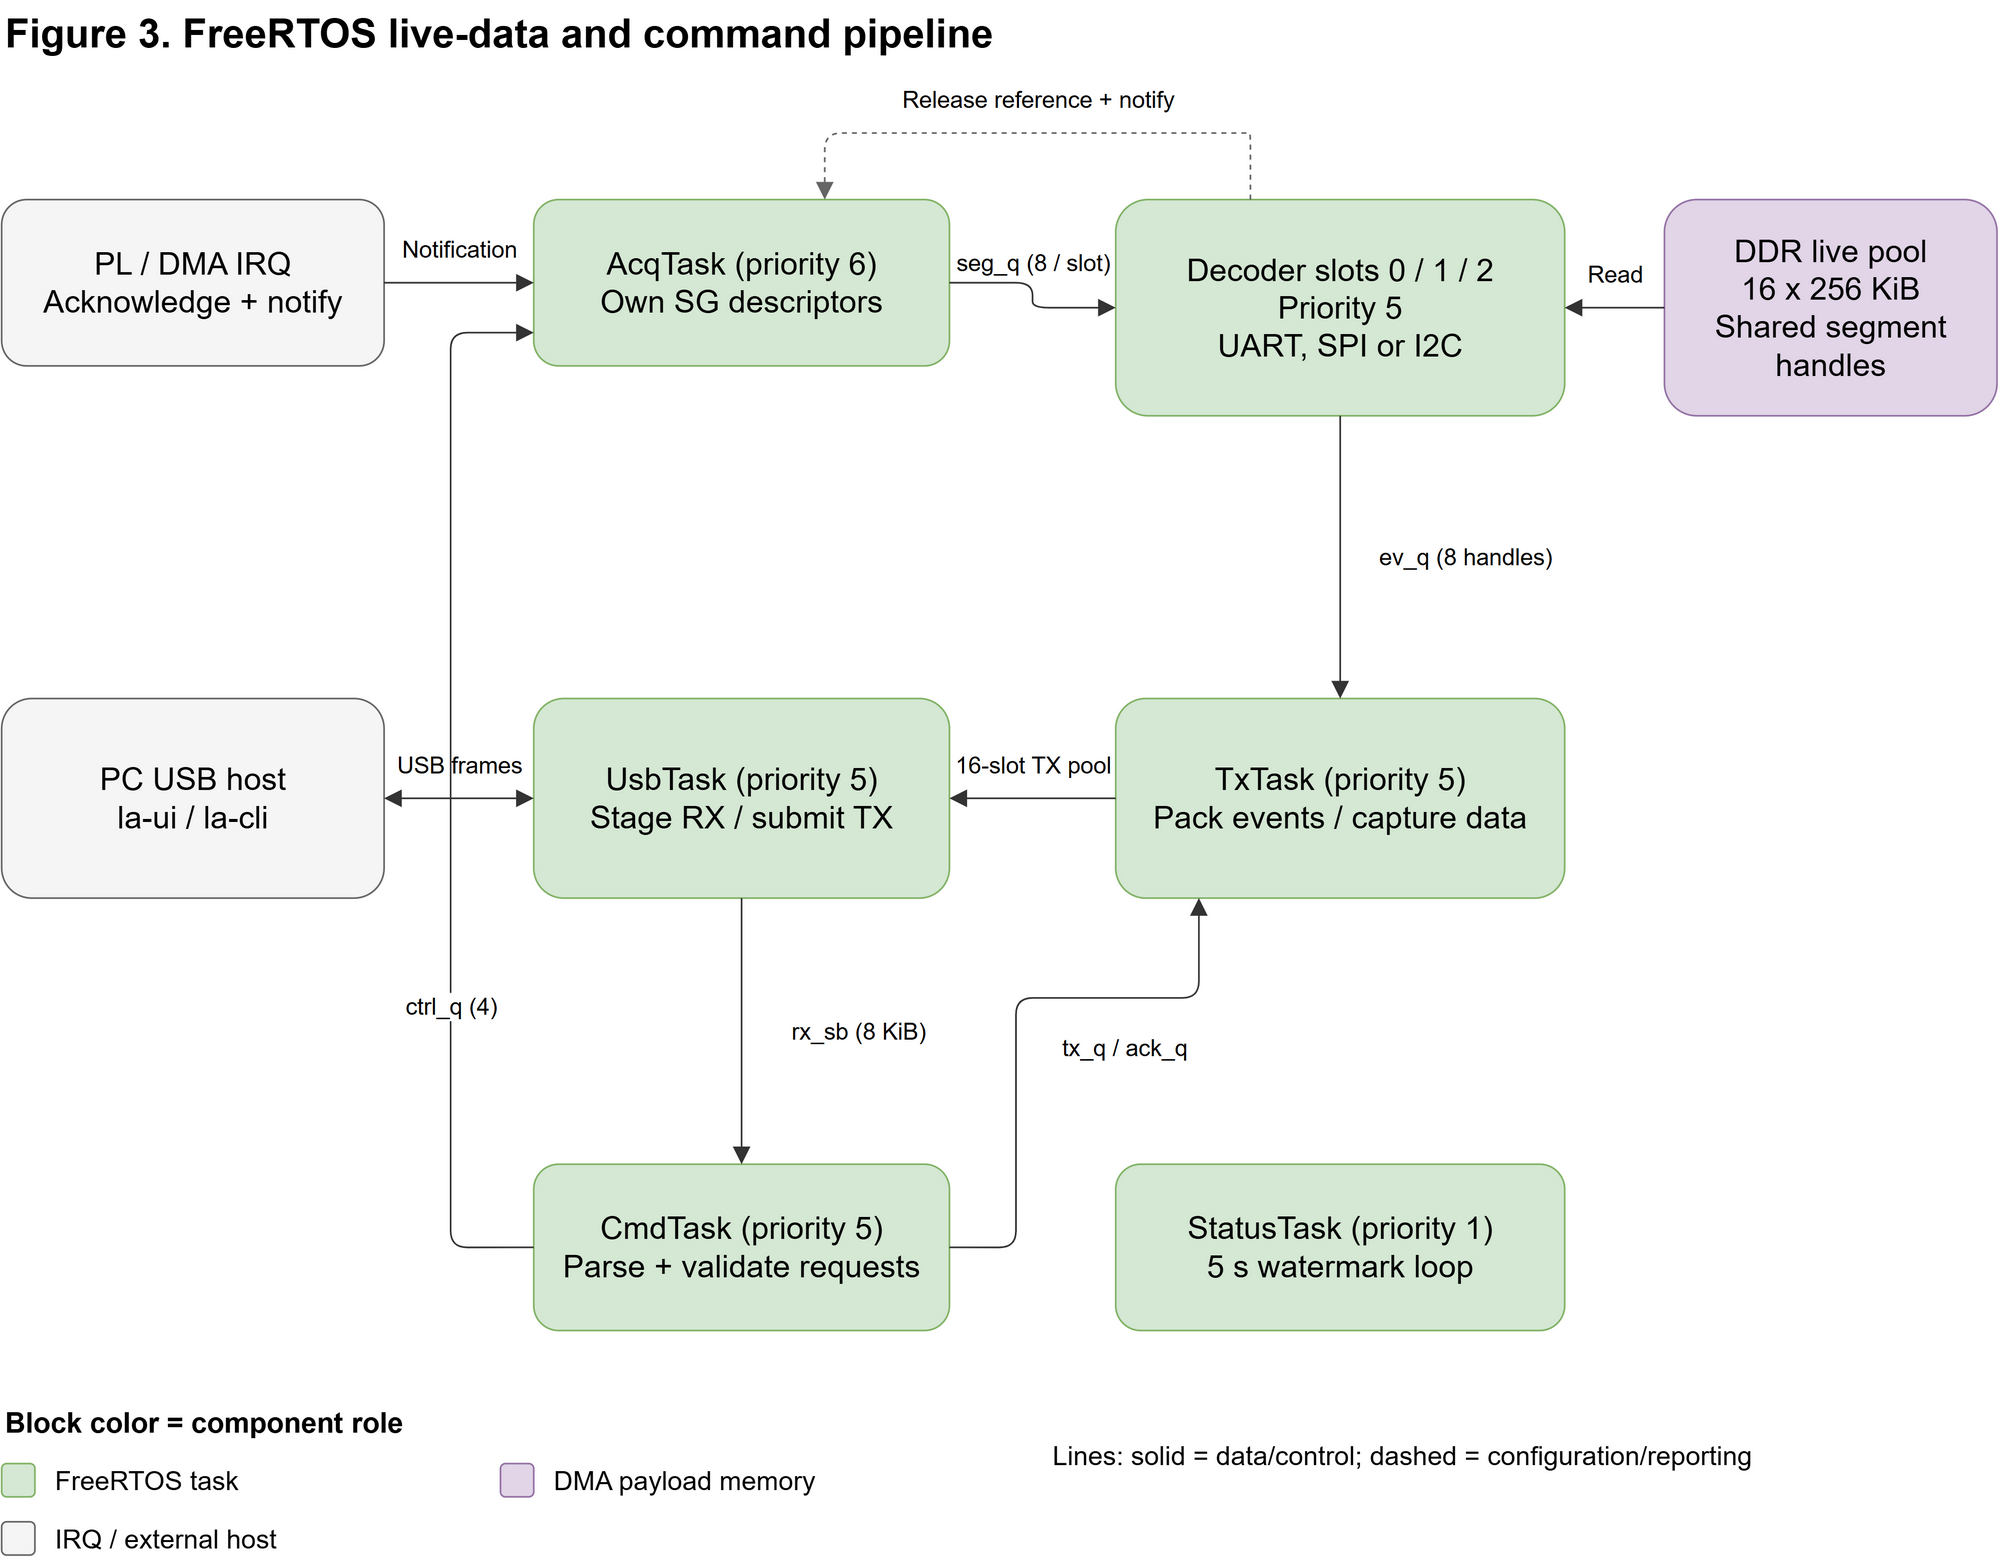
\includegraphics[width=0.85\linewidth]{../assets/figures/03-rtos.png}
\caption{RTOS data flow. AcqTask queues references to completed sample segments
for the decoder tasks. Decoders queue event blocks for TxTask. UsbTask handles
the device connection, and CmdTask handles incoming commands. StatusTask monitors
stack space in the background.}
\label{fig:rtos}
\end{figure}

For example, a live UART measurement on CH0 follows this sequence:
\begin{enumerate}[leftmargin=1.4em,itemsep=2pt,topsep=2pt]
\item The computer sends a live-start command and a UART decoder configuration.
UsbTask places received bytes in the RX stream buffer. CmdTask checks the command
frame and sends an acquisition request to AcqTask through \code{ctrl_q}.
\item AcqTask starts the live SG chain. The FPGA emits transition words
containing a 24-bit run count and an eight-bit sample value.
\item The DMA interrupt handler acknowledges completion and notifies AcqTask. AcqTask
collects completed descriptors, checks their actual lengths and invalidates the
DMA-written cache range before a decoder reads it.
\item AcqTask publishes a handle, slot, length and sequence to each enabled
decoder's \code{seg_q}. The large sample payload stays in DDR; the queue does not
copy the entire segment.
\item The configured UART task reads the segment and tracks start bits, data
bits, and stop bits across segment boundaries. It stores decoded bytes and their
sample positions in an event block. When the block fills, or the two-millisecond
flush check is due, it sends the block pointer through \code{ev_q}.
\item TxTask encodes the event frame, places it in the USB TX pool and returns
the event block to \code{block_q}. UsbTask submits ready TX slots in FIFO order;
endpoint completion returns the slot to the pool.
\item After processing the segment, a decoder releases its reference and
notifies AcqTask. Only after all consumer references are released may AcqTask
repost that segment to DMA.
\end{enumerate}

\subsubsection{Buffer sharing and synchronization}

\begin{figure}[htbp]
\centering
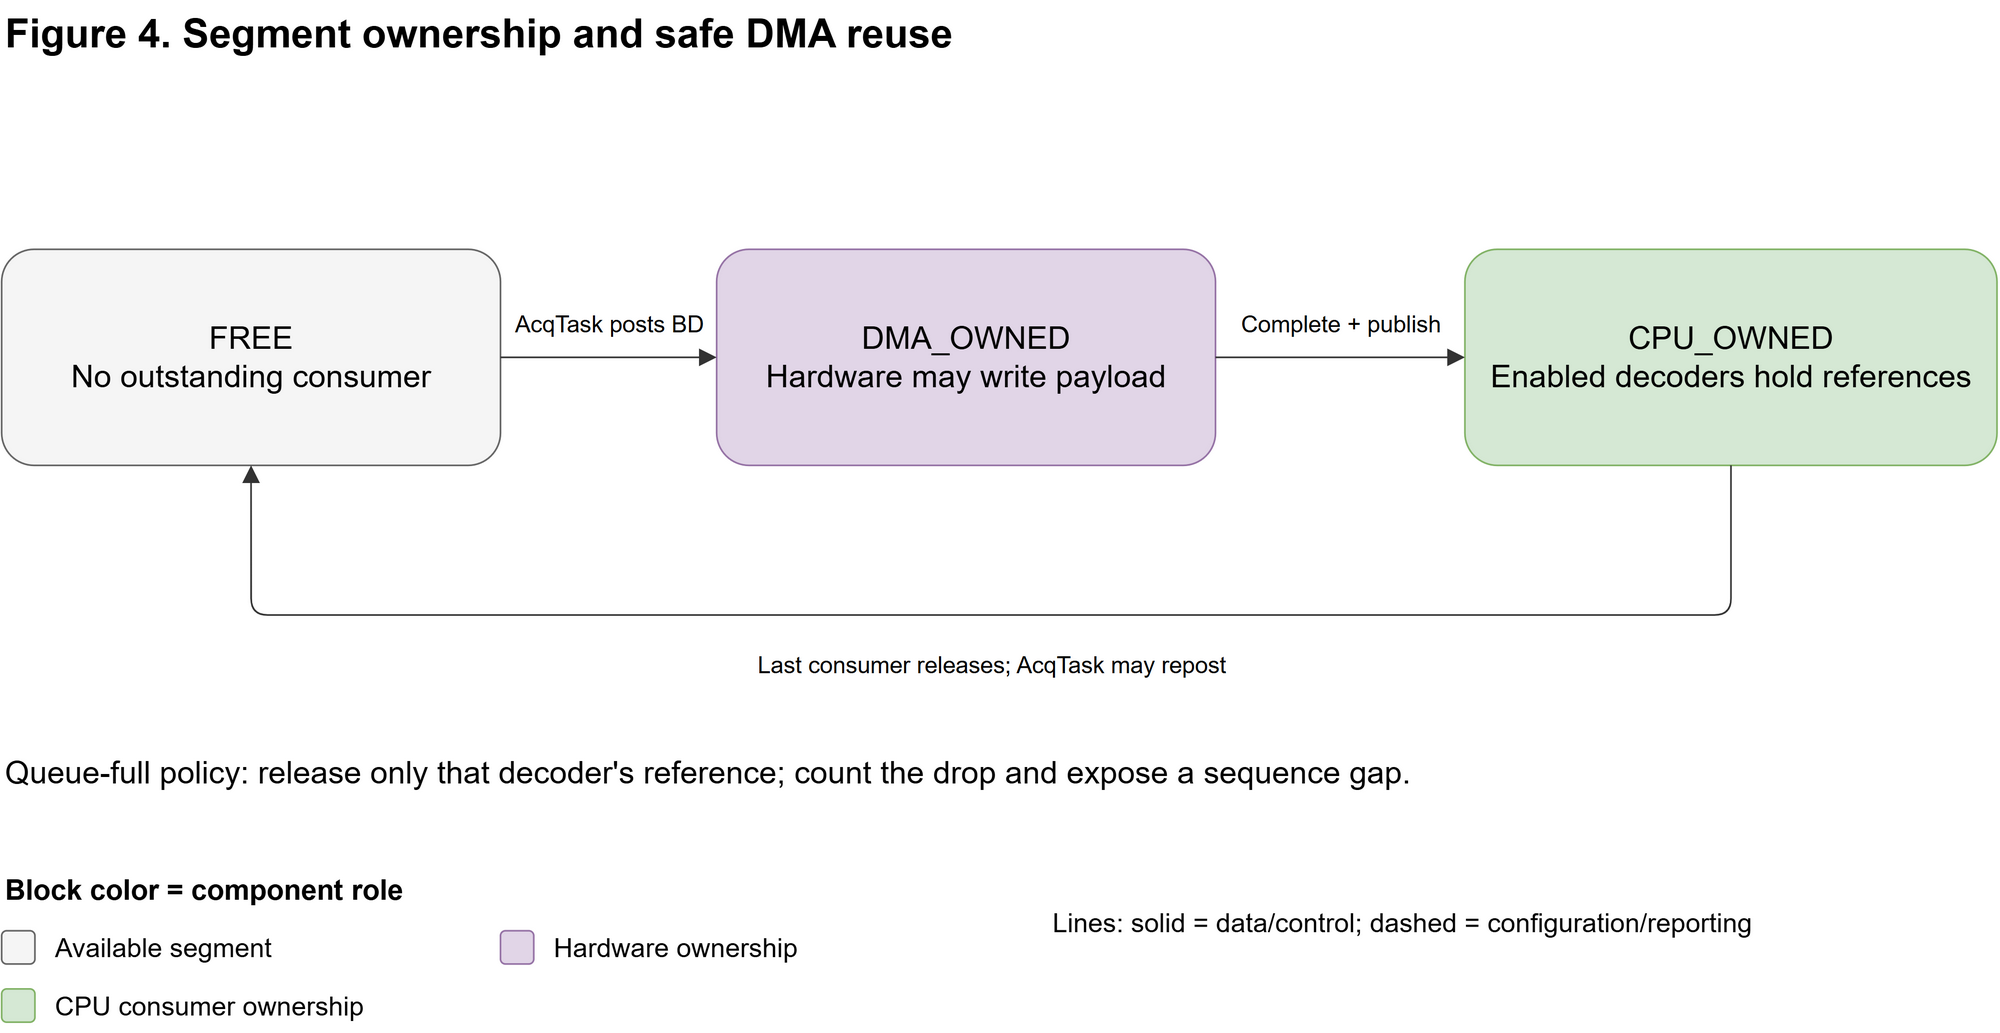
\includegraphics[width=\linewidth]{../assets/figures/04-ownership.png}
\caption{Hardware ownership and consumer ownership are exclusive. A buffer is
not returned to DMA while any enabled decoder still holds a reference.}
\label{fig:ownership}
\end{figure}

A live segment passes through three states. A \code{FREE} segment is available
for a new transfer. A \code{DMA_OWNED} segment belongs to DMA and must not be read
by a decoder. After DMA finishes, the segment becomes \code{CPU_OWNED} and can be
read by the enabled decoder tasks. It becomes free again only after every
decoder releases its reference.

This rule matters when two slots examine the same input. If one decoder finishes
before another, DMA must still wait for the slower reader before reusing that
segment. AcqTask alone changes DMA descriptors. Short critical sections protect
the shared reference counts and segment state from concurrent updates.
Generation numbers reject references to an earlier use of a buffer. Sequence
numbers reveal missing segments. After a gap, the decoder resets its protocol
state rather than joining samples from two incomplete transactions.

Queues carry commands, segment handles, or pointers to completed event blocks.
They do not copy entire sample buffers. Every queue has a fixed capacity, so the
firmware also defines what happens when producers temporarily outpace consumers.

\begin{longtable}{|>{\raggedright\arraybackslash}p{3.2cm}|>{\raggedright\arraybackslash}p{3.1cm}|>{\raggedright\arraybackslash}p{10.4cm}|}
\hline
\textbf{Queue or buffer} & \textbf{Capacity} & \textbf{Behavior when unavailable or full} \\ \hline
\endhead
\code{ctrl_q} & 4 messages & CmdTask attempts an immediate send and logs a
full queue. The USB-session abort path currently does not check send failure. \\ \hline
\code{notice_q} & 8 messages & A lifecycle notice is omitted if an immediate
send fails, allowing acquisition to continue. \\ \hline
\code{tx_q} & 16 small frames & Waits up to 20~ms, then counts a dropped frame. \\ \hline
\code{ack_q} & 32 messages & Attempts an immediate send and counts a drop on failure. \\ \hline
\code{job_q} & 1 burst job & Only one job can hold the capture buffer at a time. \\ \hline
\code{cfg_q} per slot & 2 messages & Configuration sends use a limited wait or
an immediate attempt, depending on the calling path. \\ \hline
\code{seg_q} per slot & 8 handles & Omits the new segment for that decoder and
counts the drop. Later sequence checks identify the missing data. \\ \hline
\code{block_q} & 12 static block pointers & If no free block remains, the new
event is dropped and counted. \\ \hline
\code{ev_q} & 8 filled block pointers & Drops and counts the new batch, then
returns its block for reuse. \\ \hline
USB RX stream buffer & 8~KiB & Retain the current staged input and retry when
the stream buffer is full. \\ \hline
USB RX staging & 16 entries, up to 512 bytes each & Drop the new staging entry
and count overflow when full. \\ \hline
USB TX pool & 16 $\times$ 4160-byte slots & Waits for a free-slot semaphore:
500~ms normally, or 10~ms for live events and overrun reports. Failures are counted. \\ \hline
\end{longtable}

FreeRTOS queues allow the three decoder tasks to submit event blocks safely to
one transmitter. A counting semaphore tracks the number of available USB
transmit slots. A task reserves a slot before filling it, and USB completion
returns the slot for reuse. A FIFO preserves the order of ready frames.
An atomic increment gives each frame its sequence number without competing
tasks assigning the same number.

Passing a segment handle avoids copying the sample data between tasks. It does
not eliminate all copying: decoding produces new event records, and transmission
packs those records into USB frames. If a decoder queue fills, the new segment
is omitted for that decoder and its drop count increases. Later sequence checks
expose the gap instead of presenting incomplete data as a continuous recording.

Burst mode uses the same principle for a whole capture. AcqTask sends TxTask a
\code{la_tx_job_t} containing the buffer address and length. The buffer remains
busy until TxTask sends JOB\_DONE. TxTask sends DATA\_BEGIN, DATA\_CHUNK, and
DATA\_END frames, handles acknowledgements and retransmissions, and calculates
the capture checksum. A transfer that makes no progress for two seconds can be
abandoned so that it does not reserve the capture buffer indefinitely.

\subsubsection{Interrupt work, cache handling and diagnostics}

An interrupt signals that hardware needs attention. The PL/DMA handlers in
\path{fw-zynq/app/src/drivers/la_irq.c} acknowledge the interrupt, record trace
information, and notify AcqTask through \code{xTaskNotifyFromISR()}.
\code{portYIELD_FROM_ISR()} allows the scheduler to run the awakened task when
needed. Descriptor processing, protocol decoding, and capture checksums run in
task context, keeping interrupt handling short.

The USB receive callback must also release the completed vendor-driver buffer
before the driver advances. It copies at most 512 bytes into a sixteen-entry
staging ring, releases the buffer, and notifies UsbTask. UsbTask later processes
USB setup and session work, forwards received bytes to CmdTask, checks missed
completions, and submits outgoing transfers. USB transmit completion returns a
free-slot semaphore through \code{xSemaphoreGiveFromISR()}.

The application objects are allocated statically with \code{xTaskCreateStatic()},
\code{xQueueCreateStatic()} and related APIs. BSP dynamic-allocation support
remains enabled for its kernel build, but the application task pipeline uses
static storage. The idle/timer memory hooks also supply static stacks.
Stack-overflow and malloc-failure hooks print a fatal diagnostic and halt.

The processor cache can retain an older copy of memory after DMA writes new
samples to DDR. AcqTask therefore invalidates the cache entries for each completed
live segment before giving it to a decoder. TxTask does the same before reading
a completed burst. Invalidation forces the next CPU read to obtain the updated
samples. Descriptors are non-cacheable, so descriptor accesses do not require
this step. The CPU reads sample buffers without modifying their contents.

StatusTask checks the minimum remaining stack space for acquisition, command,
transmission, and status tasks every five seconds. This stack watermark helps
identify insufficient stack allocation, although the summary does not include
every decoder or USB task. Optional trace hooks record task switches, queue
activity, DMA completion, decoding, and transmission in a fixed-size trace buffer.
The host can display these records as an RTOS timeline. Per-task CPU utilization
is not measured because kernel runtime statistics are disabled.

\subsubsection{RTOS code reference map}

\begin{longtable}{|>{\raggedright\arraybackslash}p{6.6cm}|>{\raggedright\arraybackslash}p{10.6cm}|}
\hline
\textbf{Explanation} & \textbf{Source file or group} \\ \hline
\endhead
Scheduler startup, memory checks, static kernel hooks & \path{fw-zynq/app/src/main.c} \\ \hline
Task creation and static queues/buffers & \path{fw-zynq/app/src/la_app.c} \\ \hline
Priorities, stack lengths, queue depths & \path{fw-zynq/app/src/la_app.h} \\ \hline
Tick, static allocation, overflow hooks and trace hooks & \path{fw-zynq/FreeRTOSConfig.h} \\ \hline
Descriptor ownership, live publication/repost and cache invalidation & \path{fw-zynq/app/src/tasks/la_acq_task.c} \\ \hline
Segment consumption, event batching, reference release & \path{fw-zynq/app/src/tasks/la_decoder_task.c} \\ \hline
Protocol dispatch and control routing & \path{fw-zynq/app/src/tasks/la_cmd_task.c} \\ \hline
Burst ACK window, frame packing and bounded live drain & \path{fw-zynq/app/src/tasks/la_tx_task.c} \\ \hline
USB class/session service and 1~ms wait & \path{fw-zynq/app/src/tasks/la_usb_task.c} \\ \hline
Interrupt notifications and USB receive/transmit handling &
\path{fw-zynq/app/src/drivers/la_irq.c};
\path{fw-zynq/app/src/drivers/la_usb_dev.c} \\ \hline
Pool/ring lifecycle and protocol state & \path{fw-zynq/app/src/live/}; \path{common/la_decode/} \\ \hline
Five-second monitoring loop & \path{fw-zynq/app/src/tasks/la_status_task.c} \\ \hline
\end{longtable}

Additional implementation details are available in
\path{docs/hardwarex/rtos-implementation.md}.

\section{Design files summary}

The editable project sources are organized as follows. The public code
repository is \url{https://github.com/linggaaradhanas22/logic-analyzer}.

\begin{longtable}{|>{\raggedright\arraybackslash}p{5.9cm}|>{\raggedright\arraybackslash}p{11.3cm}|}
\hline
\textbf{File group} & \textbf{Purpose} \\ \hline
\endhead
\path{fpga/rtl/}, \path{fpga/tb/}, \path{fpga/constraints/}, \path{fpga/scripts/} &
Editable RTL, self-checking testbenches, pin constraints and Vivado scripts \\ \hline
\path{docs/regmap.yaml}; \path{tools/gen_regmap.py} & Register-map source and
generated interface views \\ \hline
\path{fw-zynq/} & Vitis/FreeRTOS application, drivers, task adapters, memory
layout and build/load scripts \\ \hline
\path{common/la_proto/}; \path{common/la_decode/} & Shared C framing/integrity
code and protocol decoders \\ \hline
\path{host/la_cli/}; \path{host/la_ui/}; \path{host/la_live_web/} & CLI,
browser workspace, file handling and live-event bridge \\ \hline
\path{tests/}; \path{host/tests/}; \path{fw-zynq/tests/} & Portable, host,
integration and bench test layers \\ \hline
\path{docs/hardwarex/diagrams/}\allowbreak\code{project-report_v2.drawio} & Four
editable current system/FPGA/RTOS/ownership figures \\ \hline
\path{docs/architecture.md}; \path{docs/rtos-design.md};
\path{docs/using-the-analyzer.md}; \path{docs/status.md} & Architecture, ownership
contract, operating sequence and dated verification ledger \\ \hline
\path{fw-esp32/} & Retained optional gateway-profile implementation \\ \hline
\end{longtable}

The repository contains the editable design and test sources. Build commands
generate simulation, timing, and bench reports locally. These generated reports
must be reproduced separately after cloning the repository.

\section{Bill of materials summary}

Table prices are Indonesian-marketplace estimates from 17 September 2026.
The USB build requires the Zybo board, two USB A-to-micro-B data cables, jumper
wires, and a microSD card. One cable connects J12 for power, programming, and
console access. The other connects J10 for analyzer data. The laboratory
computer is excluded from the cost. Optional items are listed separately.

\begin{longtable}{|>{\raggedright\arraybackslash}p{1.0cm}|>{\raggedright\arraybackslash}p{8.3cm}|>{\raggedright\arraybackslash}p{1.1cm}|>{\raggedright\arraybackslash}p{2.5cm}|>{\raggedright\arraybackslash}p{2.5cm}|}
\hline
\textbf{ID} & \textbf{Component and current role} & \textbf{Qty} &
\textbf{Unit estimate (IDR)} & \textbf{Total (IDR)} \\ \hline
\endhead
A1 & Zybo Z7-10 development board, required & 1 & 13,800,000 & 13,800,000 \\ \hline
W1 & USB A-to-micro-B data cable, J12 power/JTAG/console & 1 & 25,750 & 25,750 \\ \hline
W2 & USB A-to-micro-B data cable, J10 analyzer data & 1 & 25,750 & 25,750 \\ \hline
W3 & Female-female jumper-wire pack, target leads and optional external
loopback & 1 & 20,700 & 20,700 \\ \hline
M1 & 16~GB class-10 microSD, standalone SD startup & 1 & 82,500 & 82,500 \\ \hline
PC1 & Existing Windows host computer, excluded infrastructure & 1 & 0 & 0 \\ \hline
PS1 & Optional 5~V supply; documented bench uses J12 USB power & 1 & 37,050 & 37,050 \\ \hline
A2 & Optional classic ESP32-WROOM gateway board & 1 & 45,000 & 45,000 \\ \hline
AP1 & Optional Wi-Fi access point for gateway profile & 1 & 218,000 & 218,000 \\ \hline
A3 & Optional ESP32-S3 board; historical gateway transport work & 1 & 115,000 & 115,000 \\ \hline
A4 & Optional 3.3~V USB-UART diagnostic adapter & 1 & 25,000 & 25,000 \\ \hline
BB1 & Optional solderless breakout breadboard & 1 & 13,800 & 13,800 \\ \hline
\end{longtable}

\textbf{Required USB-build subtotal: Rp 13,954,700.} This includes A1, W1, W2,
W3 and M1. Optional items total Rp 453,850; all listed items total Rp 14,408,550.
The optional power supply is not included in the required subtotal. These
figures are cost estimates rather than purchase invoices.

\subsection{Component suppliers}

Supplier references for the required components are listed below:
\begin{sloppypar}
\begin{itemize}[leftmargin=1.2em,itemsep=1pt,topsep=2pt]
\item A1: \url{https://www.tokopedia.com/invoklab/digilent-zybo-z7-zynq-7000-arm-fpga-soc-development-board-zybo-z7-10-0f6d6}
\item W1/W2: \url{https://www.tokopedia.com/robot-indonesia/robot-rdm100xs-kabel-data-micro-usb-kabel-charger-handphone-2a-panjang-1-meter-garansi-resmi-1-tahun-bisa-cod-1736307162016286082-1736307173264033154}
\item W3: \url{https://www.tokopedia.com/reinid/dupont-jumper-wire-female-to-female-kabel-40pcs-20cm-rainbow-cable-1729850275615311272}
\item M1: \url{https://www.tokopedia.com/v-genindonesia/memory-hp-maestro-microsd-16gb-maestro-class-10-chip-only}
\end{itemize}
\end{sloppypar}

No custom PCB or enclosure is needed for the documented build. The Zybo Pmod
series resistors are part of the board, not separately purchased components.

\section{Build instructions}

The project builds natively on Windows. The main tools are
Vivado/Vitis 2026.1, Questa for procedural RTL simulation, Python 3.11 and
MSVC/CMake/Ninja for portable C checks. The optional gateway uses the pinned
native ESP-IDF installation. The build commands use
\code{python tools/run.py <target>}, which locates the project from the script's
own directory.

\begin{enumerate}[leftmargin=1.5em,itemsep=2pt,topsep=2pt]
\item Clone the repository, create its \path{.venv} and install the project
package using the setup steps in \path{docs/windows-dev.md}.
\item Check the environment with
\code{python tools/run.py check-env -- --write-lock}.
\item Generate the interfaces with \code{python tools/run.py gen}.
\item Check the software with \code{python tools/run.py test-native} and
\code{python tools/run.py test-host}.
\item Simulate the RTL with \code{python tools/run.py sim} and build the
bitstream/XSA with \code{python tools/run.py bit}.
\item Build the default USB firmware with \code{python tools/run.py fw-zynq}.
\item With the documented power/jumper setup, load the design with
\code{python tools/run.py jtag-zynq}.
\item For SD startup, run \code{python tools/run.py boot}, copy BOOT.BIN to the
FAT32 card root, remove power, set JP5 to SD and power-cycle. \code{package}
stages the profile-aware firmware/host artifacts and hash manifest.
\end{enumerate}

The firmware build uses USB by default. The optional
\code{--profile gateway} argument selects the older ESP32 gateway configuration
for commands that support it.

\section{Operation instructions}

\subsection{Connections and startup}

\begin{tabularx}{\linewidth}{|>{\raggedright\arraybackslash}p{3.2cm}|>{\raggedright\arraybackslash}X|}
\hline
\textbf{Connection or setting} & \textbf{Current direct-USB configuration} \\ \hline
J12 & PC USB connection for board power/JTAG/FTDI console \\ \hline
J10 & PC USB data connection to the analyzer CDC-ACM endpoint \\ \hline
J11 & Unused in device mode \\ \hline
JP6 & USB power selection for the documented bench arrangement \\ \hline
JP1 / JP2 & Open for the documented J10 device-mode arrangement \\ \hline
JP5 & JTAG for development load, or SD for the verified standalone image \\ \hline
JC & Eight acquisition inputs, CH0--CH7, plus common ground to the target \\ \hline
JE & Pattern-generator outputs for optional external loopback \\ \hline
\end{tabularx}

\begin{enumerate}[leftmargin=1.5em,itemsep=2pt,topsep=2pt]
\item Remove power before changing jumpers or wiring. Check the board revision,
target logic voltage and shared ground. Do not connect target VCC.
\item Connect J12 for power and J10 for analyzer data. Load the USB image over
JTAG, or boot the prepared SD card with JP5 set to SD.
\item Identify J10's USB Serial Device COM port. The recorded bench used COM13;
another PC can assign a different number. Do not select J12's FTDI console.
\item Start \code{la-ui} from the project environment, or use
\path{tools/win/la-ui-start.vbs}. Open \url{http://127.0.0.1:8080/} in the
browser.
\item Rescan/select the analyzer port and Connect. Ping should report firmware
0x000A0000 and PL ID 0x4C410002 for the current W11 image.
\item Begin with the internal counter self-test before connecting target signals.
Use the UI runbook's 100~MS/s, raw, zero-pre-trigger configuration. The UI scales
step-pattern timing so the Fit view shows readable square waves.
\end{enumerate}

\subsection{Capture, decode and inspect}

Use zoom/pan/Fit, channel selection, cursors A/B, edge stepping and pattern
search to inspect recorded waveforms. Capture decoding uses the host native DLL,
built by \code{test-native}. At 10~MS/s, the pattern-generator recipes are:

\begin{tabularx}{\linewidth}{|>{\raggedright\arraybackslash}p{1.8cm}|>{\raggedright\arraybackslash}p{2.2cm}|>{\raggedright\arraybackslash}p{4.6cm}|>{\raggedright\arraybackslash}X|}
\hline
\textbf{Protocol} & \textbf{Generator mode} & \textbf{Decoder configuration} &
\textbf{Expected stimulus} \\ \hline
UART & \code{uart} & \code{uart:rx=0,baud=115200} & Repeating LA-TEST followed by
newline \\ \hline
SPI & \code{spi} & \code{spi:sck=0,mosi=1,cs=2} & Frames containing 4C 41; the
first can be partial \\ \hline
\iu{} & \code{i2c} & \code{i2c:scl=3,sda=4} & START, address/write, ACK, 4C 41,
STOP \\ \hline
\end{tabularx}

For a real target, replace generator input with appropriately wired 3.3~V
signals, keep common ground and choose a rate that resolves the signal edges.
Configure trigger/pre/post settings for the region of interest. In live mode,
configure the desired decoder slots and use Start/Stop; each enabled slot has
independent configuration. Decoded-pattern stop acts after the decoder has
processed the relevant segment, not exactly at the physical edge.

\subsection{UART demonstration}
\label{sec:uart-demo}

The following screenshots were captured on 18 October 2026 from the current W11
image (firmware 0x000A0000, PL 0x4C410002) with the analyzer connected to an
ESP32-S3 UART demonstration on CH0. The capture used 10~MS/s, 64k raw, Pre 0, no
edge trigger, Patgen off, CH0 only, and slot 0 configured as
\code{uart:rx=0,baud=115200}. The decoded bytes are
\texttt{4C 41 2D 53 33 0A} (\texttt{LA-S3\textbackslash n}). The live session
reported 1,464 events and 1,220 real waveform packets with zero gaps.

A video demonstration of the working instrument is available on YouTube:
\href{https://youtu.be/1xx84Ndi4vQ?si=ldsuYEWvYVqu2u6-}{\texttt{youtu.be/1xx84Ndi4vQ}}.

\begin{figure}[htbp]
\centering
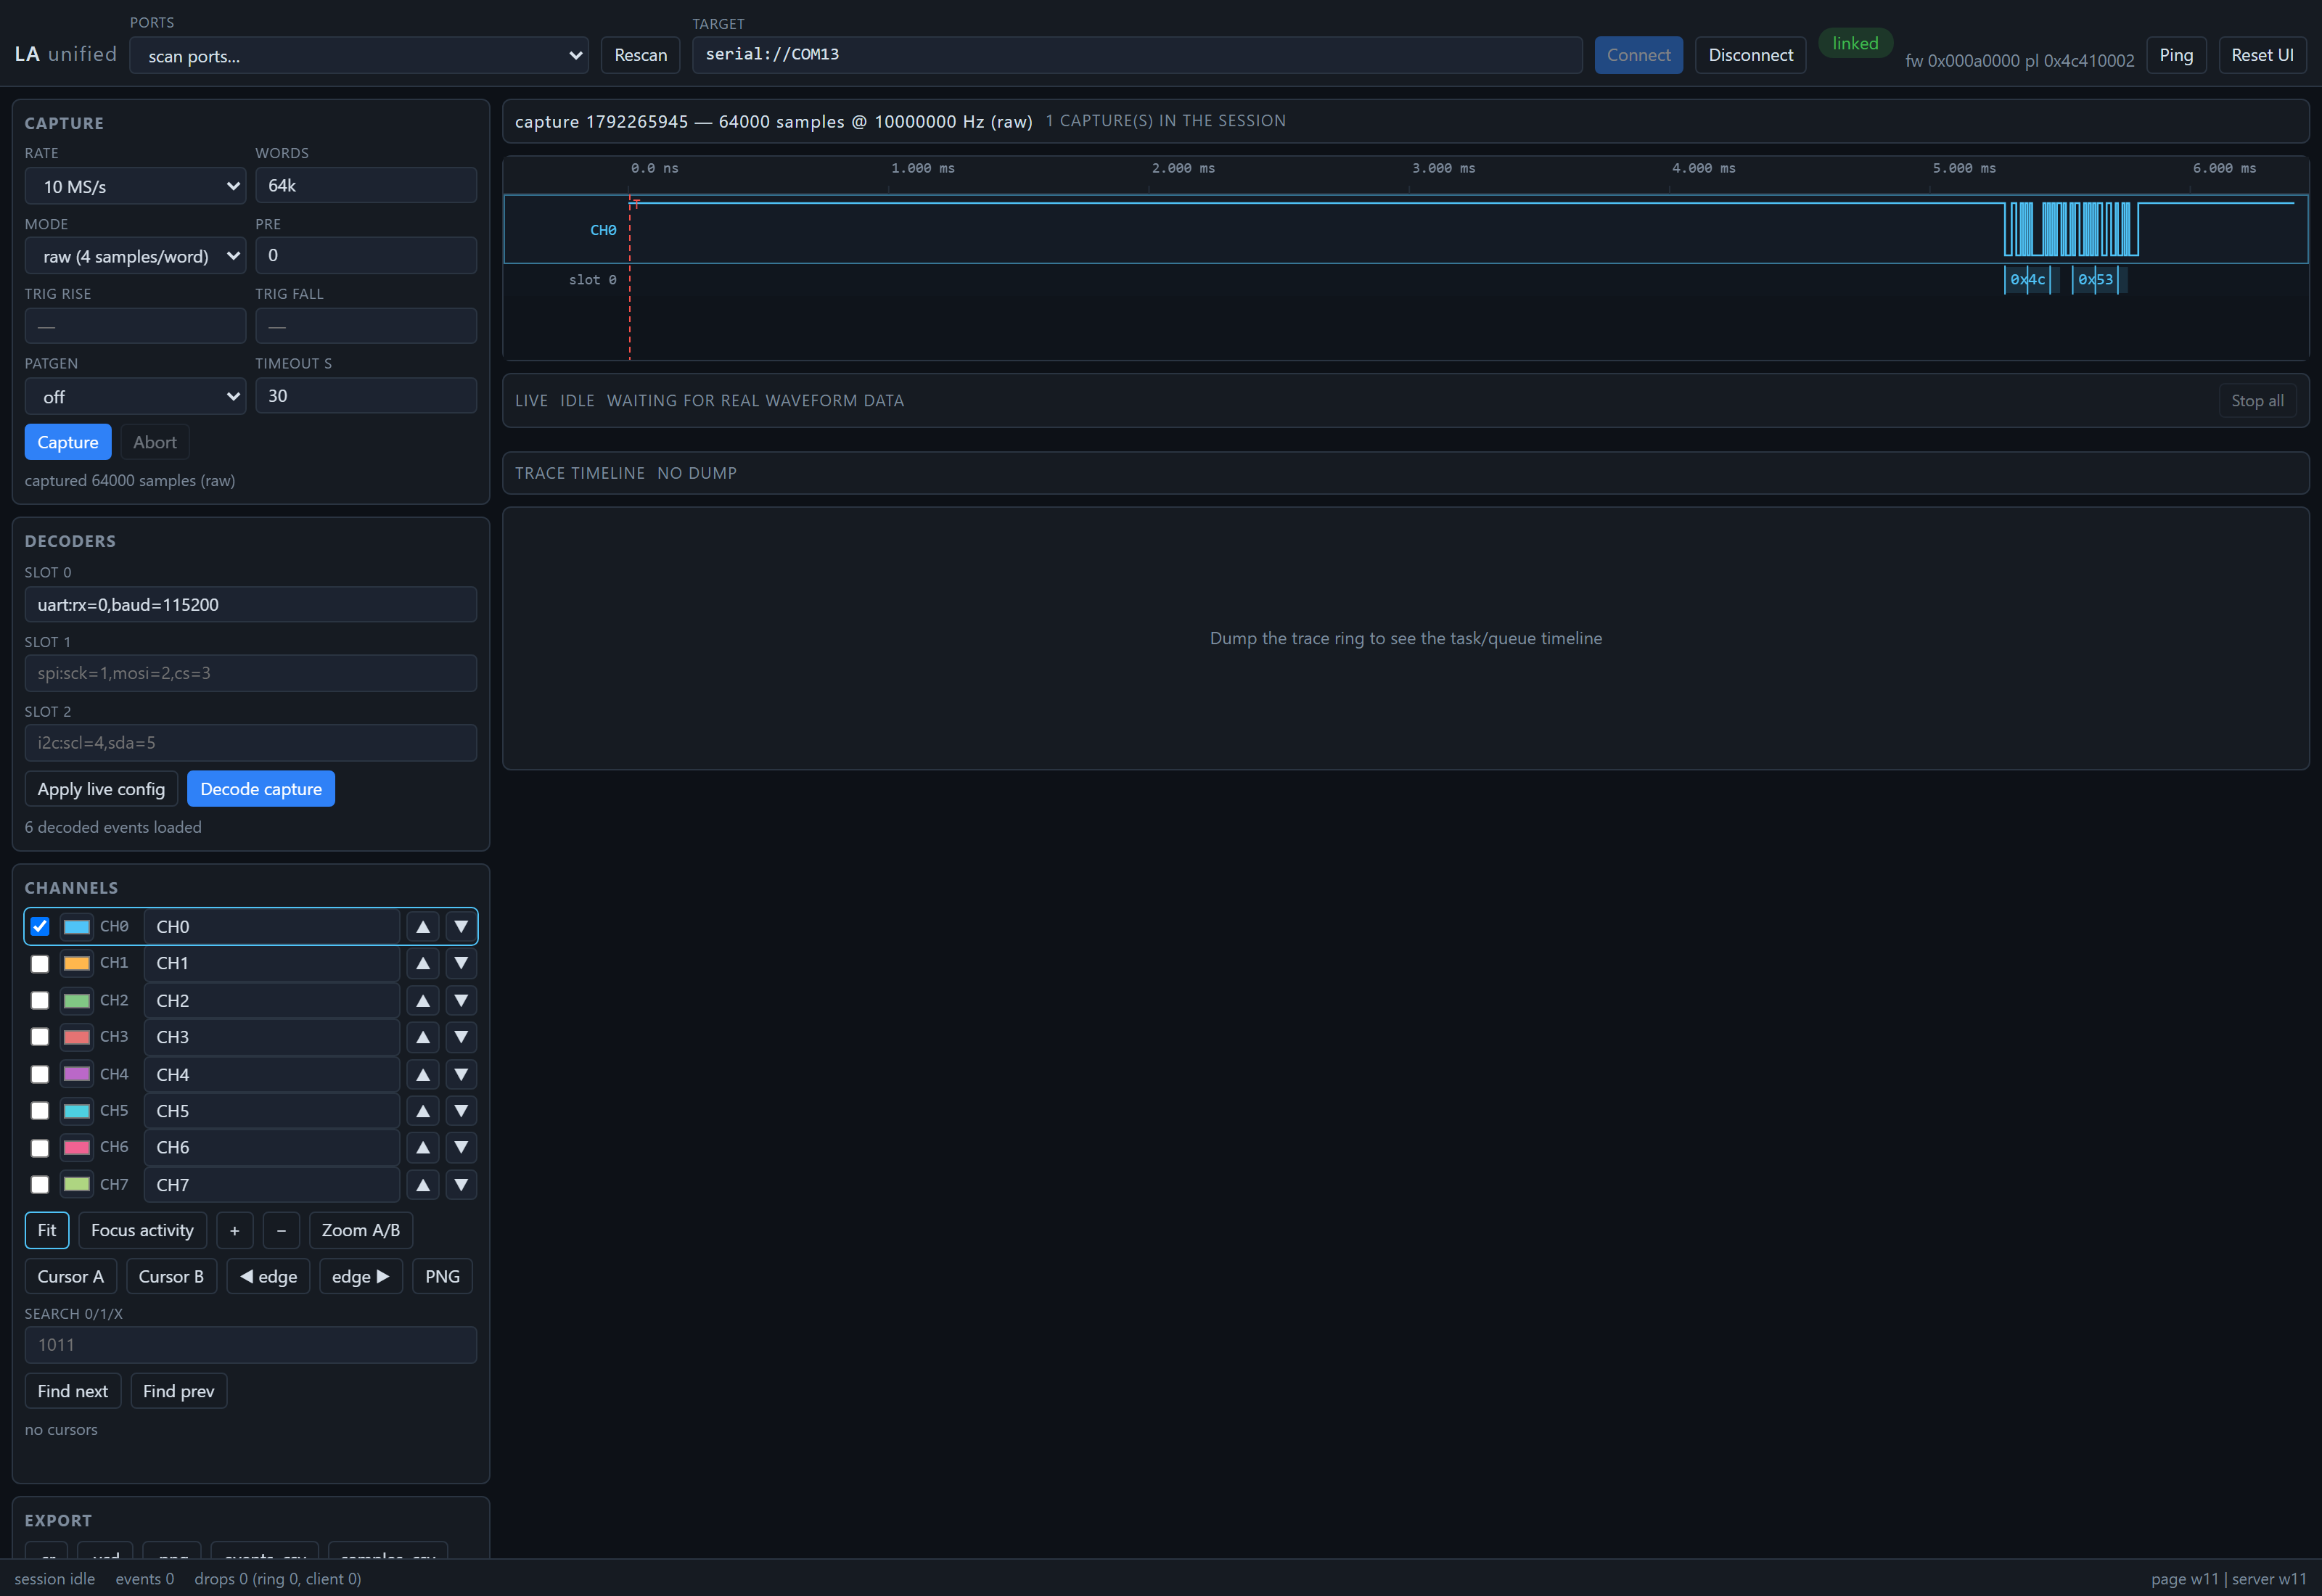
\includegraphics[width=\linewidth]{../assets/uart-demo/uart-demo-capture.png}
\caption{Logic analyzer UI connected to the UART demonstration. The capture
panel is configured for 10~MS/s, 64,000 raw samples, pre-trigger zero, no edge
trigger and pattern generator off. Slot 0 decodes UART RX on CH0 at 115200 baud,
and the waveform shows the UART frame annotations.}
\label{fig:uart-ui}
\end{figure}

\begin{figure}[htbp]
\centering
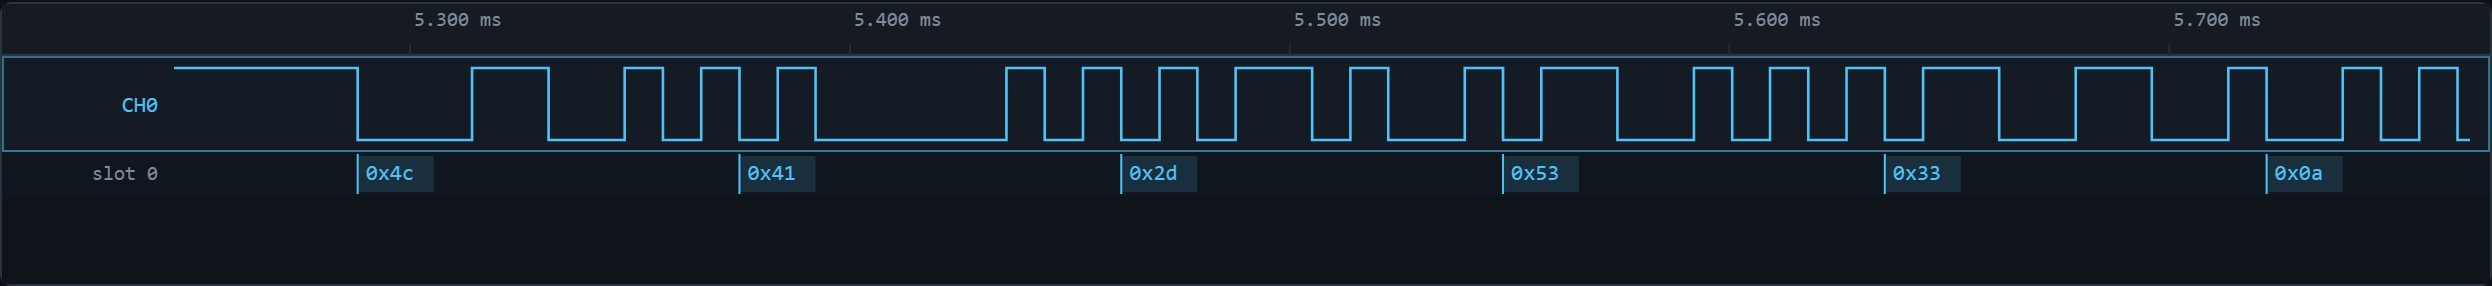
\includegraphics[width=\linewidth]{../assets/uart-demo/uart-demo-frame.png}
\caption{Close-up of the decoded UART frame. The eight data bits of each byte are
visible on CH0, and the annotations show \texttt{4C 41 2D 53 33 0A}, the bytes
for \texttt{LA-S3} followed by a newline.}
\label{fig:uart-frame}
\end{figure}

\begin{figure}[htbp]
\centering
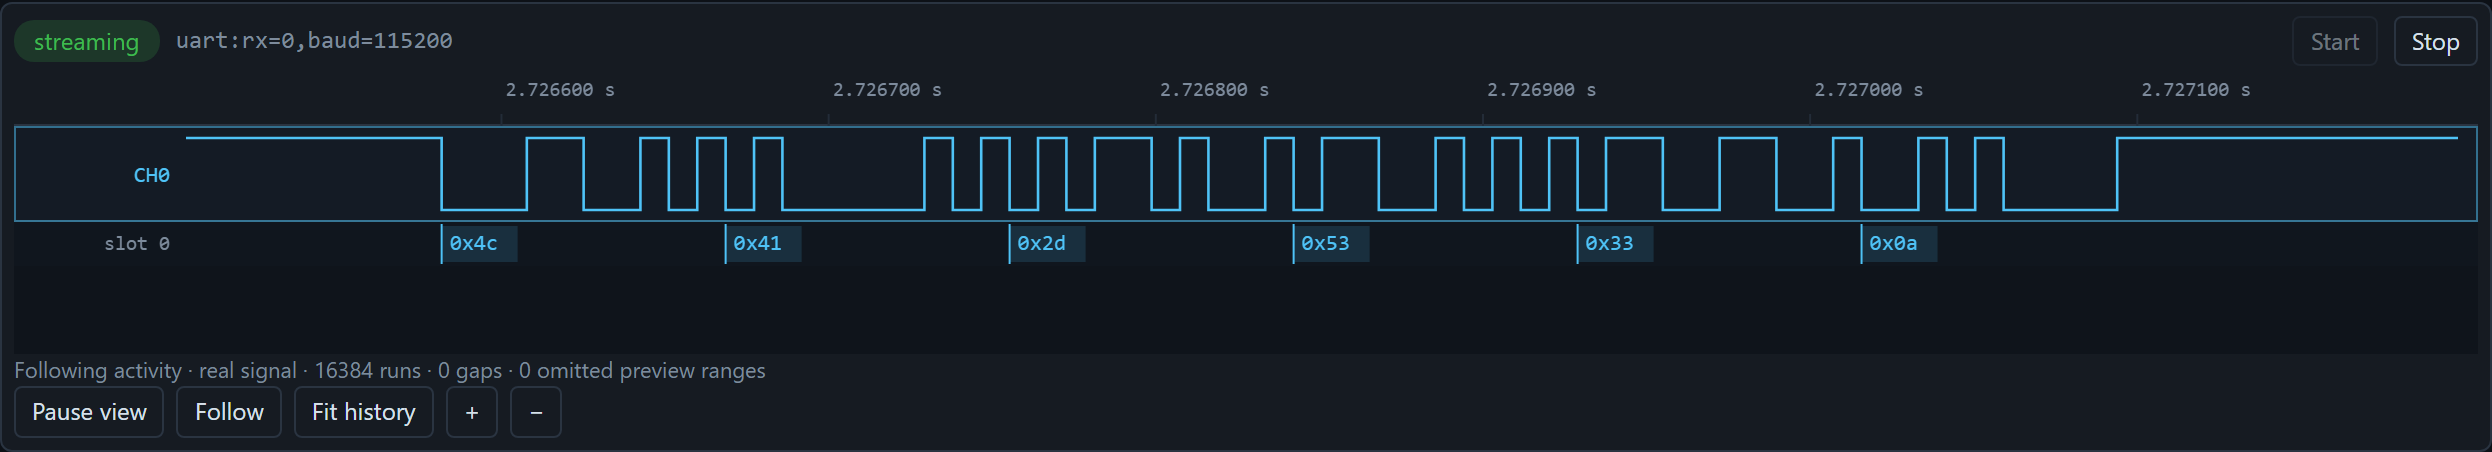
\includegraphics[width=\linewidth]{../assets/uart-demo/uart-demo-live-pane.png}
\caption{Live UART decoding in slot 0. The real waveform and decoded bytes share
one timeline; the status line reports the run count and zero gaps for the
recorded live session.}
\label{fig:uart-live}
\end{figure}

\subsection{Export and shutdown}

Export \code{.sr} for exact sample-count reopening in PulseView or the UI. VCD
stores transitions and may not preserve a trailing constant run's exact sample
count; the host reports this limitation. Sample CSV contains waveforms, while
event CSV contains decoded annotations. PNG captures the visible waveform region.
Trace controls retrieve the RTOS timeline. Stop live operation, finish/cancel
jobs, disconnect the UI, stop its host server and remove power before rewiring.

All acquisition inputs are 3.3~V only and have no project-added over-voltage
protection. Use an appropriate external level shifter for 5~V logic. Short leads
and common ground are important; synchronization does not guarantee capture of
pulses shorter than the configured sample period.

\section{Validation and characterization}

\subsection{Test methods and results}

Verification covered the FPGA logic, acquisition data, USB transfer, protocol
decoding, and browser operation. Self-checking RTL simulations compared logic
outputs against expected results. Internal pattern-generator tests exercised
the acquisition pipeline, while external loopback tests also checked the board
connections. USB tests compared received bytes and checksums with expected data.
Live tests checked event counts, sequence gaps, and recovery after overload.

The table gives the results and test dates. Earlier gateway-era measurements are
identified separately because they do not measure the present USB connection.
The UART demonstration in Section~\ref{sec:uart-demo} uses firmware 0x000A0000
and PL 0x4C410002.

\begin{longtable}{|>{\raggedright\arraybackslash}p{3.9cm}|>{\raggedright\arraybackslash}p{7.0cm}|>{\raggedright\arraybackslash}p{5.9cm}|}
\hline
\textbf{Test} & \textbf{Result} & \textbf{Report or date} \\ \hline
\endhead
Procedural RTL regression & 12/12 self-checking Questa cases passed in the
recorded regressions & \path{fpga/tb/testlist.json}; \path{docs/status.md} and
simulation reports \\ \hline
Routed FPGA resources & 6,675/17,600 LUTs (37.93\%); 9,198/35,200 registers
(26.13\%); 37/60 BRAM tiles (61.67\%) & \path{build/release/utilization.rpt},
20 September 2026 \\ \hline
Routed timing & Setup WNS +0.576~ns; hold WHS +0.022~ns; no failing constrained
endpoints & Routed timing summary, 20 September 2026 \\ \hline
Capture matrix & Six generator modes at 1, 10 and 100~MS/s, three captures each;
internal and full eight-channel external matrices recorded as 18/18 & Historical
P6/P7 matrix entries in \path{docs/status.md} \\ \hline
USB aggregate drain & Three trials, each 67,108,864 bytes as 16 $\times$ 4~MiB
captures; 41.4--41.5~s; 1.62~MB/s; byte-exact/CRC-clean &
\path{build/reports/usb-u06-performance.md}, 19 September 2026 \\ \hline
USB UART live delivery & 606,411 device events and browser-feed events in 60~s;
606,405 decoded bytes; 124.7~kB/s wire; zero client/format drops, overrun events
or dropped segments & \path{build/reports/usb-v04-live-web.md} and V04 ledger
entry, 20 September 2026 \\ \hline
USB live protocols/recovery & UART, 10~kHz SPI/\iu{}, stop-on-pattern, compact
events, overload recovery and close/reopen checks; 8/8 tests passed & V04/V06
USB live suites, 20 September 2026 \\ \hline
UI real-device integration & 6/6 API/E2E cases; million-sample capture, decoding,
per-slot live/SSE, trace/export/offline open & W09 entry, 20 September; SD-boot
re-run, 26 September 2026 \\ \hline
Cached decoder comparison & Approximately 1.28--1.29~M transition words/s, about
28\% faster than non-cached under deliberate SPI overload &
\path{docs/rtos-design.md} P8.5, 12 September 2026 \\ \hline
Historical isolated-byte latency & 428 microseconds worst over 20 single-shot
sessions against a 25~ms budget & P7.6/P8.2 evidence; earlier Zynq/link scope \\ \hline
Historical capture soak & 500 back-to-back 4096-sample captures, exact results
and no FIFO overflow, 232~s & P8.4 recorded soak evidence \\ \hline
Software regression & Release precheck 22/22; host regression 180/180;
native regression 18/18 & Release reports and 18 October 2026 relocation checks
in \path{docs/status.md} \\ \hline
USB-profile SD boot & BOOT.BIN cold boot, USB enumeration, ping/status and 6/6 UI
E2E cases & \path{build/reports/sd-boot-verification.md}, 26 September 2026 \\ \hline
Current-image SD boot & Cold boot with firmware 0x000A0000; USB UI tests 6/6;
external UART browser checks 10/10 & \path{build/reports/sd-w11/},
18 October 2026 \\ \hline
\end{longtable}

The routed design meets its internal timing constraints at 100~MHz. The positive
setup and hold margins indicate that constrained internal paths meet their
required timing. External-I/O delay warnings remain in the report, so these
results do not establish timing margins for every target circuit or probe setup.

The USB trial transferred 64~MiB in total through sixteen separate 4~MiB
captures. It did not require a 64~MiB capture buffer. Its 1.62~MB/s result measures
transfer of stored data, whereas 100~MS/s describes sampling inside the FPGA.
These rates explain why full-speed raw acquisition must be buffered.

The cached-decoder comparison deliberately overloaded SPI decoding. Both cached
and non-cached cases dropped segments, so the measured improvement describes
processing throughput under overload. The earlier 428-microsecond latency result
measures a different link configuration, not USB-to-browser latency. In the
60-second UART test, zero client loss refers to the active browser-feed consumer.
The host can still discard old replay history when its history buffer fills.

\subsection{UART demonstration results}

The external UART demonstration links a known transmitted message to both a
recorded waveform and live decoded events. The ESP32-S3 sends
\texttt{LA-S3\textbackslash n} at 115200 baud. At 10~MS/s, each UART bit spans
approximately 87 samples, allowing the decoder to resolve the frame timing.
The captured result contains the expected six bytes, and the live run reports
zero sequence gaps. The screenshots show the signal on CH0, the decoded frame,
and the live display. This checks the complete path from an external input
through acquisition and decoding to the browser.

\subsection{Capabilities and remaining limitations}

\begin{itemize}[leftmargin=1.4em,itemsep=2pt,topsep=2pt]
\item The tested sampling rate is up to 100~MS/s on eight 3.3~V channels.
The proposed 200~MS/s extension remains unverified.
\item Burst capacity is bounded by the 8~MiB pool and finite descriptor chain;
oversized captures are rejected rather than silently shortened.
\item Live tests cover UART at 115200 baud and SPI/\iu{} at 10~kHz. Faster
inputs can exceed decoder or transport capacity. Drop counters and sequence-gap
reports identify missing data.
\item Full-rate raw capture is buffered acquisition, not a 100~MB/s continuous
USB stream. The default host drain measurement is 1.62~MB/s.
\item The optional ESP32 gateway still has Wi-Fi/SPI throughput limitations
and an unresolved ESP32-S3 SPI issue. Direct USB bypasses that transport path.
\item Direct SUMP integration is deferred because it depends on a signed
driver. PulseView analysis is available through exported \code{.sr} files.
\end{itemize}

\section{Conclusion}

The logic analyzer captures eight digital channels at up to 100~MS/s and supports
triggered captures, pre-trigger history, and UART, SPI, and \iu{} decoding.
The FPGA maintains sampling timing, while DMA moves the data into memory.
FreeRTOS coordinates the next stages through task priorities, notifications,
queues, and buffer reference counts. This arrangement allows acquisition,
decoding, USB transmission, and command handling to progress concurrently
without reusing a buffer before its readers finish.

USB tests achieved 1.62~MB/s for stored capture transfer. The live UART test
delivered 606,411 events in 60 seconds without dropped segments or client loss.
These results support buffered high-speed measurement and live analysis within
the tested protocol rates. They also show the main design trade-off: the FPGA
can acquire data faster than the processor and USB link can continuously deliver
it. Finite captures, transition encoding, and reported data gaps manage that
difference.

\section*{Author contributions}

\ifFPGA
Lingga Aradhana Sahadewa is the lead author and contributor for this FPGA
submission, responsible for overall system design, remaining FPGA work,
embedded and host software, integration, testing, and documentation.
Alvin Hadar contributed RTL design for the
capture FIFO/buffer and sample packing. Bagas Budhi Permana contributed RTL
design for trigger/edge detection and AXI-Stream packet framing.
\else
Lingga Aradhana Sahadewa is the sole author and contributor for this Embedded
system submission, including system design, FPGA and embedded implementation,
host software, integration, testing, and documentation.
\fi

\section*{Acknowledgements}

This project was funded by the Korea Chamber of Commerce and Industry (KCCI).
\ifFPGA
The authors thank KCCI for supporting the FPGA class project.
\else
The author thanks KCCI for supporting the Embedded system class project.
\fi

\section*{References}

\begin{enumerate}[leftmargin=1.5em,itemsep=2pt,topsep=2pt]
\item Project code, specifications and dated execution ledger:
\url{https://github.com/linggaaradhanas22/logic-analyzer};
\path{docs/status.md}, \path{docs/architecture.md},
\path{docs/rtos-design.md} and \path{docs/using-the-analyzer.md}.
\item Digilent, Zybo Z7 reference documentation:
\url{https://digilent.com/reference/programmable-logic/zybo-z7/start}.
\item AMD, Vivado/Vitis and AXI DMA documentation: \url{https://docs.amd.com/};
the actual routed utilization/timing reports dated 20 September 2026.
\item FreeRTOS kernel and scheduling documentation: \url{https://www.freertos.org/};
the project's configuration and source files listed in Section~\ref{sec:rtos}.
\item sigrok/PulseView signal-analysis ecosystem: \url{https://sigrok.org/}.
\item Saleae logic analyzers: \url{https://www.saleae.com/}; Digilent Digital
Discovery: \url{https://digilent.com/shop/digital-discovery-portable-logic-analyzer-and-pattern-generator/}.
\end{enumerate}

\appendix
\section{Weekly project activity summary}

The class-project period is 15 September--12 October 2026. The following summary
matches the four weekly logs in the accompanying KCCI workbook, with five hours
allocated to each week. Earlier technical tests are cited in the results section
under their original dates. The 18 October UART screenshots and SD-image checks
are supplementary verification after the class-project period.

\begin{longtable}{|>{\raggedright\arraybackslash}p{1.3cm}|>{\raggedright\arraybackslash}p{3.2cm}|>{\raggedright\arraybackslash}p{10.4cm}|>{\raggedright\arraybackslash}p{1.3cm}|}
\hline
\textbf{Week} & \textbf{Period} & \textbf{Activity and outcome summary} &
\textbf{Hours} \\ \hline
\endhead
1 & 15--21 September 2026 & Defined the channel, sample-rate, trigger, and protocol
requirements. Designed the FPGA--DMA--DDR--FreeRTOS--PC architecture, register
interface, sample formats, and buffer-ownership rules. Selected direct USB and
created the implementation and verification plan.
& 5 \\ \hline
2 & 22--28 September 2026 & Implemented input synchronization, the sample divider,
triggers, pre-trigger storage, and capture control. Added raw/run packing,
the output FIFO, and AXI-Stream packet framing. Connected registers, DMA,
interrupts, DDR access, and board pins. Checked RTL behavior, routed timing,
and resource use. & 5 \\ \hline
3 & 29 September--5 October 2026 & Created FreeRTOS tasks, queues, and static
buffers. Implemented DMA descriptor handling, interrupt notifications, cache
maintenance, and buffer reference counts. Integrated UART/SPI/\iu{} decoder
slots, USB framing and recovery, and host capture, waveform, cursor, and export
controls. & 5 \\ \hline
4 & 6--12 October 2026 & Integrated the FPGA, firmware, and host tools and checked
SD startup. Verified captures with internal patterns and external loopback.
Checked live decoding, overload reporting, stop/abort, and USB recovery.
Reviewed performance against requirements, refined the viewer, and completed
the diagrams, report, presentation, and operating instructions. & 5 \\ \hline
Total & Four-week project period & Four weekly logs & 20 \\ \hline
\end{longtable}

Detailed weekly activity logs are provided on four separate sheets in the
accompanying KCCI workbook.

\end{document}
